\subsection{Application of Model}

\par To apply the model to real-world competitions, we construct two world-class virtual time trialists: MTT (Male Time Trialist) and FTT (Female Time Trialist), together with their power profiles. Then we use the model to simulate the process of their participation in real-world competitions. After finding the best tactic through numerical optimization, their results will be compared with real-world competitors.

\par Power profiles of MTT and FTT are listed as table [\ref{tab:pp}]:
% Table generated by Excel2LaTeX from sheet 'timetrialist'
% Table generated by Excel2LaTeX from sheet 'timetrialist'
\begin{table}[htbp]
	%	\renewcommand\arraystretch{1.3}
	\setlength{\belowcaptionskip}{0.2cm}
	%\setlength\tabcolsep{16pt}%调列距
	\centering
	\caption{ Power Profiles of MTT and FTT}
	\begin{tabular}{c|cccc|cccc}
		\toprule[2pt]
		& \multicolumn{4}{c|}{MTT}      & \multicolumn{4}{c}{FTT} \\
		\midrule
		maximum duration & 5 s   & 1 min & 5 min & FT    & 5 s   & 1 min & 5 min & FT \\
		power output(W/kg) & 19.69 & 10.01 & 6.98  & 6.40  & 17.48 & 9.29  & 6.33  & 5.61 \\
		\bottomrule[2pt]
	\end{tabular}%
	\label{tab:pp}%
\end{table}%

\subsubsection{2021 Olympic Time Trial course in Tokyo}
% TODO: \usepackage{graphicx} required
\begin{figure}[h]
	\centering
	\includegraphics[width=0.8\linewidth]{"image/东京+uci/东京 女 time trial circuit"}
	\caption{Topographic profile of 2021 Olympic Time Trial course in Tokyo}
	\label{trackt}
\end{figure}
\paragraph{} Tracks of 2021 Olympic Time Trial in Tokyo are both around Mount Fuji, and both courses have a lot of elevation fluctuations. The women will complete one full lap for a total of 22.1 kilometers with a total elevation gain of 423 meters[\ref{trackt}], and the men cover a distance of 44.2 kilometers, which is two laps around the women's track.

\par We use the power profile of MTT and FTT, and we apply our model to this course. As the terrain of the course is very undulating, it's hard to ignore the effects of altitude changes on athletes, so we take it into account. With the help of our model, we get the minimum time to cover the distance for to virtual athletes, shown in table [\ref{time}].
% Table generated by Excel2LaTeX from sheet 'Sheet2'
\begin{table}[htbp]
	%	\renewcommand\arraystretch{1.3}
	\setlength{\belowcaptionskip}{0.2cm}
	\setlength\tabcolsep{16pt}%调列距
	\centering
	\caption{ Minimum time to finish OITT}
	\begin{tabular}{ccccc}
		\toprule[2pt]
		&$ T_1$(min)    & $T_2$(min)    & $T_3$ (min)   & Total(min) \\
		\midrule
		MTT   & 28:41 & 21:15 & 7:16  & 57:12\\
		FTT   & 22:39 & 3:17  & 8:42  & 34:38\\
		\bottomrule[2pt]
	\end{tabular}%
	\label{time}%
\end{table}%
\par As is shown in table [\ref{time}], the virtual male rider exerts his strength at the level of FTP in the first 28:41(min), and recover for 21:16(min), controlling his average power output per kg at 6.40 W/kg. in the final sprint, he exerts all effort over the level of FTP, maintaining 7.16 power output per kg, and finally scores 57:12(min). The same goes for the analysis of women, whose power output per kg is FTP, 5.61 and 6.34 separately.
\par In order to verify the correctness of the model, we compare the score of  MTT with that of three riders who participated in 2021 Olympic Time Trial, and find that our MTT and FTT rider rank 7 and 23 separately. As our data simulates the level of world athletes, our optimization results are reliable.
% TODO: \usepackage{graphicx} required
\begin{figure}[h]
	\centering
	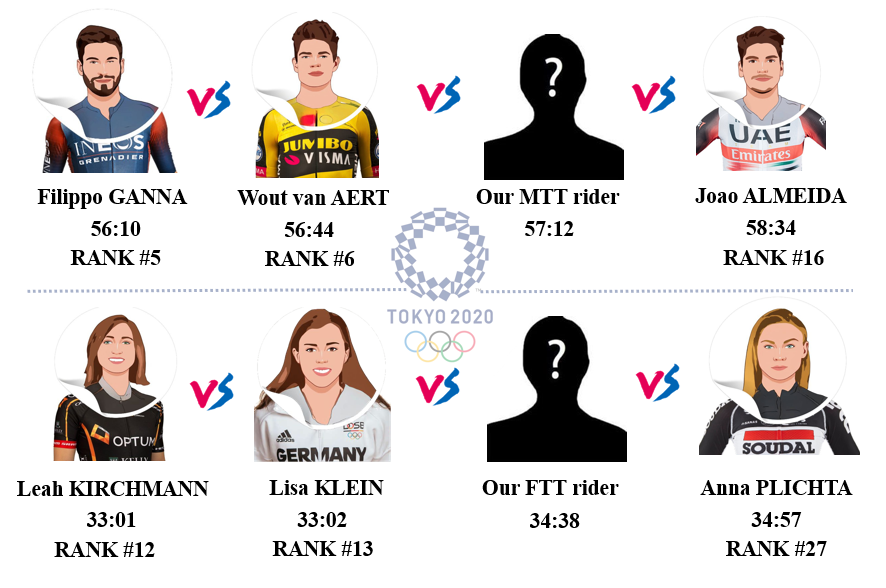
\includegraphics[width=0.8\linewidth]{image/tkyo}
	\caption{Our virtual riders and participants of 2021 Olympic Time Trial}
	\label{tkyo}
\end{figure}
 
\subsubsection{2021 UCI World Championship time trial course in Flanders}
\paragraph{} The start of 2021 UCI World Championship time trial is situated on the North Sea beach for both men and woman elite. The women will complete course for a total of 30.30 kilometers with a total elevation gain of 54 meters and men need to finish additional lap for 13 kilometers and elevation gain of 24 meters compared with women's. The whole course is relatively flat which belongs to Cat 4 comparing with Hors Catégorie. Therefore, the energy consumption per kilometer is considered the same under the windless condition on flat ground, which means $E(s)$ always equals $\overline{E}$.
\par By applying our model, we obtain the minimum time to finish race for virtual athletes, shown in table [\ref{time2}].
\begin{table}[h]
	%	\renewcommand\arraystretch{1.3}
	\setlength{\belowcaptionskip}{0.2cm}
	\setlength\tabcolsep{16pt}%调列距
	\centering
	\caption{ Minimum time to finish UCI WCTT}
	\begin{tabular}{ccccc}
		\toprule[2pt]
		&$ T_1$(min)    & $T_2$(min)    & $T_3$ (min)   & Total(min) \\
		\midrule
		MTT   & 27:23 & 15:07 & 7:05  & 49:35 \\
		FTT   & 26:21 & 3:17  & 8:49  & 38:27 \\
		\bottomrule[2pt]
	\end{tabular}%
	\label{time2}%
\end{table}%

\par As is shown in table [\ref{time2}], our virtual male cyclist applies power at the level of FTP in the first 27:23(min), the recovers for 14:07(min)and finally makes all-out effort to the end. His total result is 48:36(min). Results of female cyclist can be interpreted similarly.
\begin{figure}[h]
	\centering
	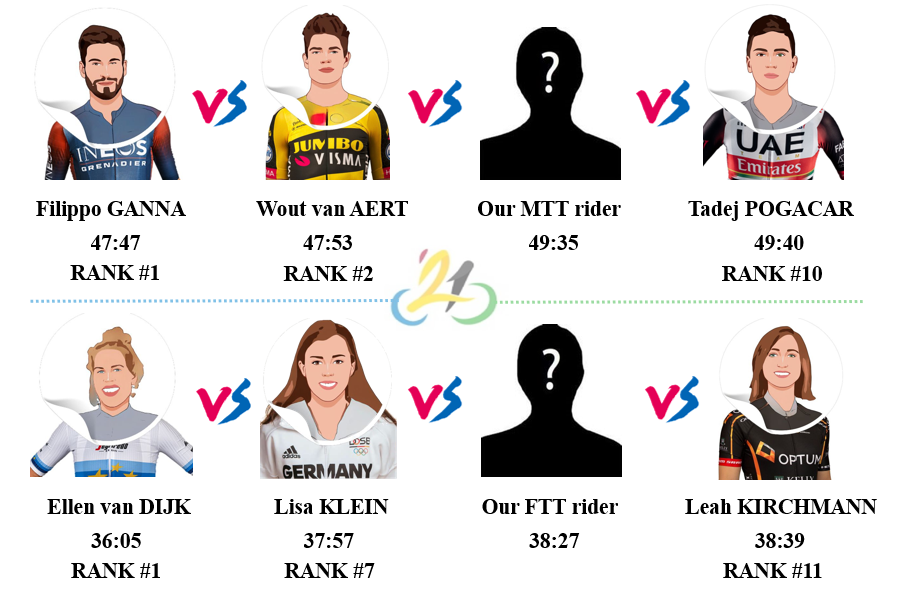
\includegraphics[width=0.9\linewidth]{image/rider1}
	\caption{Our virtual riders and participants of 2021 UCI World Championship time trial}
	\label{rider1}
\end{figure}
\par In order to verify the rationality and reliability of our model, we compare the score with ITT racers in 2021 UCI World Championship time trial as the graph presented [\ref{rider1}]---our MTT and FTT rider rank 5 and 10 respectivly.
% TODO: \usepackage{graphicx} required


\subsubsection{Self-designed course}

\paragraph{} By researching and sifting through a large number of cycling routes, we optimize one route which satisfies almost every requirements\footnote{https://www.strava.com/activities/1178477346/overview}. This course [\ref{route}] is located in Berkeley, USA, passing through Greezly Peak and Berkeley Hills and finanlly ending up back at Berkeley. Riders will complete this course with many sharp curves and nontrivial road grades for a total of 28.26 kilometers with a total elevation gain of 564 meters.
% TODO: \usepackage{graphicx} required
\begin{figure}[h]
	\centering
	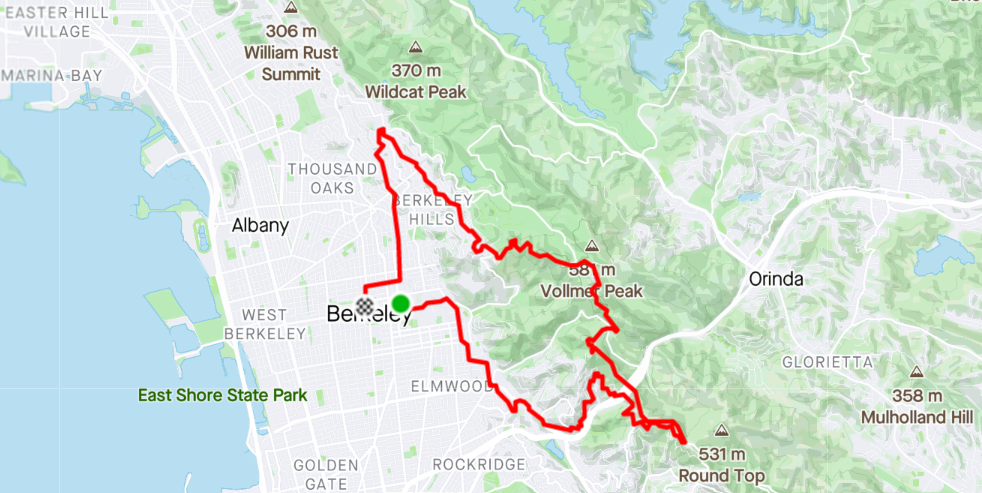
\includegraphics[width=1\linewidth]{image/route}
	\caption{Self-designed route}
	\label{route}
\end{figure}

\par From the circuit profile, after setting off, riders will head on a continuous uphill reaching 4.5 per cent gradient on average[\ref{self1}]. Then, the rolling roads include other climbs which are gentler than the previous course. After reaching the peak, riders will face downhill of almost 10 kilometers along the twists and turns to the finish.
% TODO: \usepackage{graphicx} required
\begin{figure}[h]
	\centering
	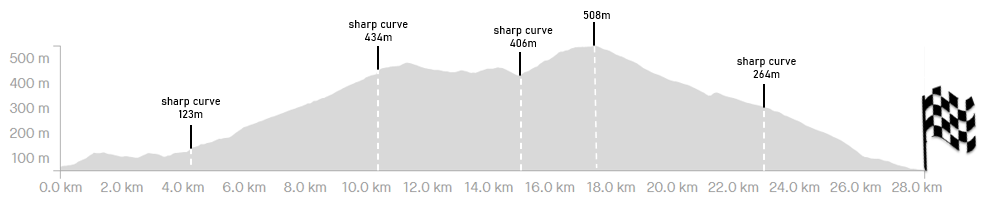
\includegraphics[width=0.9\linewidth]{image/self1}
	\caption{Topographic profile of self-designed course}
	\label{self1}
\end{figure}
\par By applying our model into our self-designed route, the optimal ride planning can be derived [\ref{time3}]. 
\begin{table}[h]
	%	\renewcommand\arraystretch{1.3}
	\setlength{\belowcaptionskip}{0.2cm}
	\setlength\tabcolsep{16pt}%调列距
	\centering
	\caption{ Minimum time to finish self-designed course}
	\begin{tabular}{ccccc}
		\toprule[2pt]
		&$ T_1$(min)    & $T_2$(min)    & $T_3$ (min)   & Total(min) \\
		\midrule
    MTT   & 28:51 & 5:37  & 7:14  & 41:42 \\
FTT   & 32:55 & 5:41  & 8:49  & 47:25 \\
\bottomrule[2pt]
\end{tabular}%
\label{time3}%
\end{table}%
\par Also, an amateur completed the track and uploaded his ride stats on the website. We compare the simulated data to his ride data [\ref{rider3}], and find that the rider lags behind our MTT and FTT riders. It's easy to explain: our riders are world-class athletes, while the strava user is an  amateur. As a result, our model can be correctly applied and proved again. 
% TODO: \usepackage{graphicx} required
\begin{figure}[h]
	\centering
	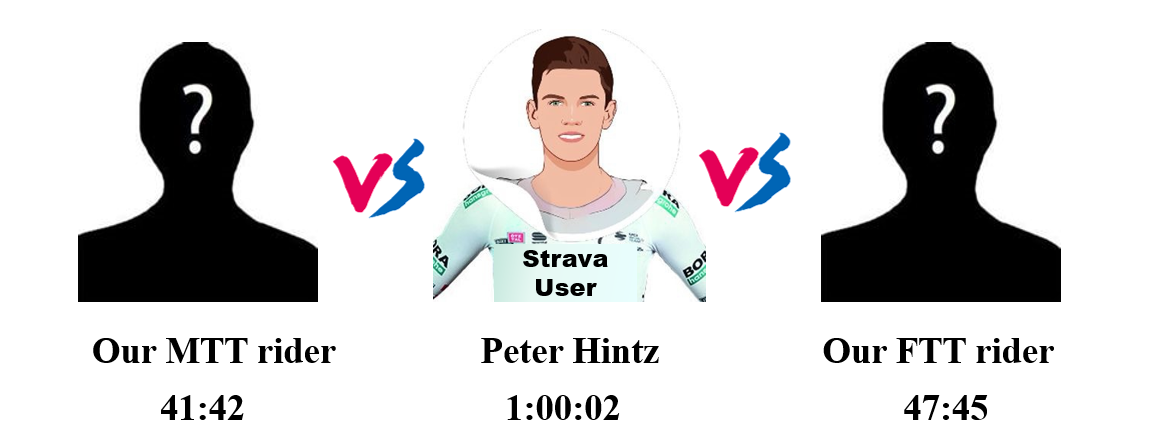
\includegraphics[width=0.7\linewidth]{image/rider3}
	\caption{Our virtual riders and participants of self-designed time trial}
	\label{rider3}
\end{figure}
